%%%%%%%%%%%%%%%%%%%%%%%%%%%%%%%%%%%%%%%%%%%%%%%%%%%%%%%%%%%%%%%%%%%%%%%%%%%%%%%%
%%                                                                
%%      SWSC LaTeX class for Journal of Space Weather and Space Climate
%%      
%%                                      (c) Springer-Verlag HD
%%                                      revised by EDP Sciences
%%                                      further revised by J. Watermann 
%%
%%%%%%%%%%%%%%%%%%%%%%%%%%%%%%%%%%%%%%%%%%%%%%%%%%%%%%%%%%%%%%%%%%%%%%%%%%%%%%%%
%%
%%      This demonstration file was derived from aa.dem
%%  
%%      AA vers. 7.0, LaTeX class for Astronomy & Astrophysics
%%      demonstration file
%%                                                (c) Springer-Verlag HD
%%                                                revised by EDP Sciences
%%
%%%%%%%%%%%%%%%%%%%%%%%%%%%%%%%%%%%%%%%%%%%%%%%%%%%%%%%%%%%%%%%%%%%%%%%%%%%%%%%%
%%
%%      modified for Journal of Space Weather and Space Climate
%%      by Jurgen Watermann, Editorial Advisor to SWSC
%%
%%      01-04-2012
%%      02-04-2012 revision 1
%%      12-07-2012 revision 2
%%      06-12-2012 revision 3 
%%      01-01-2014 revision 4
%%      06-03-2014 revision 4.1
%%
%%%%%%%%%%%%%%%%%%%%%%%%%%%%%%%%%%%%%%%%%%%%%%%%%%%%%%%%%%%%%%%%%%%%%%%%%%%%%%%%
%%
%%      The two sub-figures referenced in this template are of eps and png type,
%%      respectively, in order to demonstrate the usepackages subfigure and
%%      epstopdf and thus create pdf-only output 
%%
%%      If you want to use TexLive or MikTex together with a bibtex bibliography 
%%      file you may run Latex2e from the command line 
%%          pdflatex -shell-escape swsc.tex
%%          bibtex swsc (do not include an extension such as .tex or .bib)
%%          pdflatex -shell-escape swsc.tex
%%          pdflatex -shell-escape swsc.tex
%%
%%      A double call to pdflatex after calling bibtex is necessary in order to
%%      set citations and references correctly and insure that foreward/backward  
%%      linkage (backref option) is properly applied
%%      If you use MikTex you may need to make a triple call to pdflatex
%%
%%      If you are using TexLive or MikTex but not a bibtex type of bibliography
%%      you may simply run Latex2e twice from the command line 
%%          pdflatex -shell-escape swsc.tex
%%          pdflatex -shell-escape swsc.tex
%%
%%%%%%%%%%%%%%%%%%%%%%%%%%%%%%%%%%%%%%%%%%%%%%%%%%%%%%%%%%%%%%%%%%%%%%%%%%%%%%%%
%%
%%   single column 12-point version for review
%%

%%  with traditional abstract
\documentclass[referee,a4paper,12pt,traditabstract]{swsc} 

%%  with structured abstract 
%\documentclass[referee,a4paper,12pt,structabstract]{swsc} 

\usepackage{graphicx}
\usepackage{txfonts}
\usepackage{subfigure}
\usepackage{epstopdf}
\usepackage{lineno}
\usepackage[authoryear,round]{natbib}
\usepackage[backref]{hyperref}
\usepackage{url}

%%    This version assumes using bibtex with the swsc bibliography style file
\bibliographystyle{swsc}

\hypersetup{colorlinks=true,citecolor=cyan,urlcolor=cyan,linkcolor=blue}

%%%%%%%%%%%%%%%%%%%%%%%%%%%%%%%%%%%%%%%%%%%%%%%%%%%%%%%%%%%%%%%%%%%%%%%%%%%%%%%%

\begin{document}

\begin{linenumbers}

   \title{Hydrodynamics of giant planet formation}

   \subtitle{I. Overviewing the $\kappa$-mechanism}
   
   \titlerunning{Giant planet formation}

   \authorrunning{Wuchterl and Ptolemy}

   \author{G. Wuchterl
          \inst{1}
          \and
          C. Ptolemy\inst{2}\fnmsep\thanks{Just to show the usage
          of the elements in the author field}
          }

   \institute{Institute for Astronomy (IfA), University of Vienna,
              T\"urkenschanzstrasse 17, A-1180 Vienna\\
              \email{\href{mailto:wuchterl@amok.ast.univie.ac.at}{wuchterl@amok.ast.univie.ac.at}}
         \and
             University of Alexandria, Department of Geography\\
             \email{\href{mailto:c.ptolemy@hipparch.uheaven.space}{c.ptolemy@hipparch.uheaven.space}}
             \thanks{The university of heaven temporarily does not
                     accept e-mails}
             }

%%   \date{Received September 15, 1996; accepted March 16, 1997}

  % \abstract{}{}{}{}{}        %% uncomment if structured abstract is desired
 %% 5 {} token are mandatory
 
  \abstract
 %% context heading (optional). leave {} empty if necessary  
   {To investigate the physical nature of the `nuc\-leated instability' of
   proto giant planets, the stability of layers
   in static, radiative gas spheres is analysed on the basis of Baker's
   standard one-zone model.
   %}        %% uncomment if structured abstract is selected
 %% aims heading (mandatory)
   %{        %% uncomment if structured abstract is selected
   It is shown that stability
   depends only upon the equations of state, the opacities and the local
   thermodynamic state in the layer. Stability and instability can
   therefore be expressed in the form of stability equations of state
   which are universal for a given composition.
   %}        %% uncomment if structured abstract is selected
 %% methods heading (mandatory)
   %{        %% uncomment if structured abstract is selected
   The stability equations of state are
   calculated for solar composition and are displayed in the domain
   $-14 \leq \lg \rho / \mathrm{[g\, cm^{-3}]} \leq 0 $,
   $ 8.8 \leq \lg e / \mathrm{[erg\, g^{-1}]} \leq 17.7$. These displays
   may be used to determine the one-zone stability of layers in stellar
   or planetary structure models by directly reading off the value of
   the stability equations for the thermodynamic state of these layers,
   specified by state quantities as density $\rho$, temperature $T$ or
   specific internal energy $e$.
   Regions of instability in the $(\rho,e)$-plane are described
   and related to the underlying microphysical processes.
   %}        %% uncomment if structured abstract is selected
 %% results heading (mandatory)
   %{        %% uncomment if structured abstract is selected
   Vibrational instability is found to be a common phenomenon
   at temperatures lower than the second He ionisation
   zone. The $\kappa$-mechanism is widespread under `cool'
   conditions.
   %}        %% uncomment if structured abstract is selected
 %% conclusions heading (optional), leave {} empty if necessary 
   }        %% replace by pair of curly brackets, {}, if structured abstract is selected
   

   \keywords{giant planet formation --
                $\kappa$-mechanism --
                stability of gas spheres
               }

   \maketitle
%%
%%________________________________________________________________

\section{Introduction}

%%  This two-panel figure was inserted by JFW to demonstrate the subfigure and epstopdf packages

   \begin{figure}
   \centering
   \subfigure{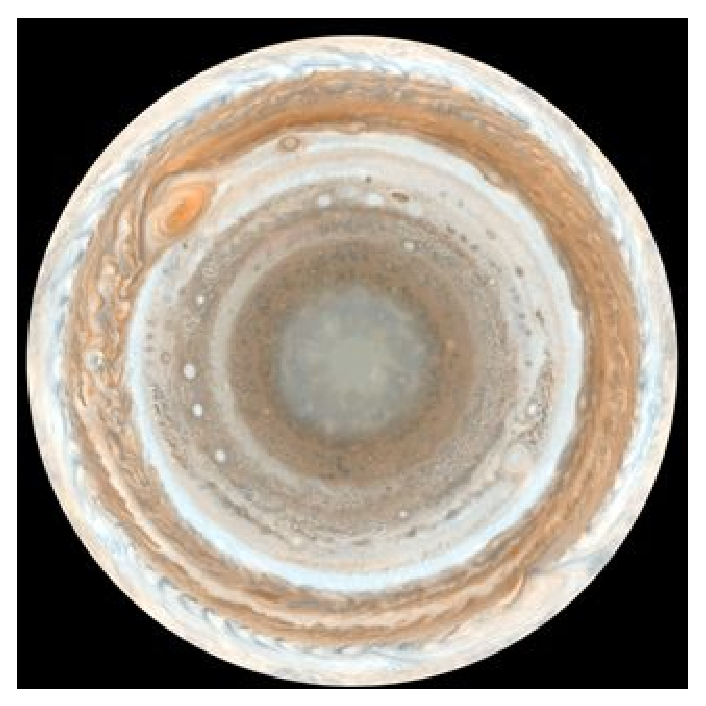
\includegraphics[width=0.6\columnwidth]{jupiter_aurora_cassini.eps}}
   \vspace{12pt}
   \subfigure{\includegraphics[width=0.6\columnwidth]{saturn_aurora_hubble.png}}
   \caption{\small Colour maps of the two largest known gas planets in the solar system.
            Top panel: Polar stereographic projection showing Jupiter's 
            south pole in the center and its equator at the edge. 
            The map was constructed from images taken by the Cassini spacecraft 
            in December 2000 as it passed Jupiter on its way to Saturn 
            (Image courtesy NASA/JPL/Space Science Institute).
            Bottom panel: Saturn displaying aurora, photographed by the Hubble Space Telesope 
            on 28 January 2004 
            (Image courtesy of NASA, ESA, J. Clarke (Boston University), and Z. Levay (STScI)).} 
   \label{fig:JupSat}
   \end{figure}

   In the \emph{nucleated instability\/} (also called core
   instability) hypothesis of giant planet formation, a critical mass for 
   static core envelope protoplanets has been found. \citet{mizuno} 
   determined the critical mass of the core to be about $12 \,M_\oplus$
   ($M_\oplus=5.975 \times 10^{27}\,\mathrm{g}$ is the Earth mass), 
   which is independent of the outer boundary
   conditions and therefore independent of the location in the
   solar nebula. This critical value for the core mass corresponds
   closely to the cores of today's giant planets (see Fig.~\ref{fig:JupSat} 
   for images of the two largest known gas planets in the solar system).

   Although no hydrodynamical study has been available many workers
   conjectured that a collapse or rapid contraction will ensue after 
   accumulating the critical mass. The main motivation for this article
   is to investigate the stability of the static envelope at the
   critical mass. With this aim the local, linear stability of static
   radiative gas  spheres is investigated on the basis of Baker's
   standard one-zone model \citep{baker}. 

   Phenomena similar to the ones described above for giant planet
   formation have been found in hydrodynamical models concerning star
   formation where protostellar cores explode \citep{{tscharnuter},{balluch}},
   whereas earlier studies found quasi-steady collapse flows. The
   similarities in the (micro)physics, i.e., constitutive relations of
   protostellar cores and protogiant planets serve as a further
   motivation for this study.

   Phenomena very different from, even entirely opposite to, the ones described
   above were recently reported by \citet{fool} and \citet{fou} who developed 
   a new model which was, however, subsequently proven to be self-contradictory 
   \citep{{dummkopf},{aaron15}}.


\section{Baker's standard one-zone model}

   In this section the one-zone model of \citet{baker},
   originally used to study the Cephe{\"{\i}}d pulsation mechanism, will
   be briefly reviewed. The resulting stability criteria will be
   rewritten in terms of local state variables, local timescales and
   constitutive relations.

   \citet{baker} investigates the stability of thin layers in
   self-gravitating, spherical gas clouds with the following properties:
   \begin{itemize}
      \item hydrostatic equilibrium,
      \item thermal equilibrium,
      \item energy transport by grey radiation diffusion.
   \end{itemize}
   For the one-zone-model Baker obtains necessary conditions
   for dynamical, secular and vibrational (or pulsational)
   stability (Eqs.\ (34a,\,b,\,c) in \citet{baker}. Using Baker's
   notation:
   \[
      \begin{array}{lp{0.8\linewidth}}
         M_{r}  & mass internal to the radius $r$     \\
         m               & mass of the zone                    \\
         r_0             & unperturbed zone radius             \\
         \rho_0          & unperturbed density in the zone     \\
         T_0             & unperturbed temperature in the zone \\
         L_{r0}          & unperturbed luminosity              \\
         E_{\mathrm{th}} & thermal energy of the zone
      \end{array}
   \]
\noindent
   and with the definitions of the \emph{local cooling time\/}
   \begin{equation}
      \tau_{\mathrm{co}} = \frac{E_{\mathrm{th}}}{L_{r0}} \,,
   \end{equation}
   and the \emph{local free-fall time}
   \begin{equation}
      \tau_{\mathrm{ff}} =
         \sqrt{ \frac{3 \pi}{32 G} \frac{4\pi r_0^3}{3 M_{\mathrm{r}}}}\,,
   \end{equation}
   Baker's $K$ and $\sigma_0$ have the following form:
   \begin{eqnarray}
      \sigma_0 & = & \frac{\pi}{\sqrt{8}}
                     \frac{1}{ \tau_{\mathrm{ff}}} \\
      K        & = & \frac{\sqrt{32}}{\pi} \frac{1}{\delta}
                        \frac{ \tau_{\mathrm{ff}} }
                             { \tau_{\mathrm{co}} }\,;
   \end{eqnarray}
   where $ E_{\mathrm{th}} \approx m (P_0/{\rho_0})$ has been used and
   \begin{equation}
   \begin{array}{l}
      \delta = - \left(
                    \frac{ \partial \ln \rho }{ \partial \ln T }
                 \right)_P \\
   \end{array}
   \end{equation}
   is a thermodynamical quantity which is of order $1$ and equal to $1$
   for nonreacting mixtures of classical perfect gases. The physical
   meaning of $ \sigma_0 $ and $K$ is clearly visible in the equations
   above. $\sigma_0$ represents a frequency of the order one per
   free-fall time. $K$ is proportional to the ratio of the free-fall
   time and the cooling time. Substituting into Baker's criteria, using
   thermodynamic identities and definitions of thermodynamic quantities,
   \begin{displaymath}
      \Gamma_1      = \left( \frac{ \partial \ln P}{ \partial\ln \rho}
                           \right)_{S}    \, , \;
      \chi^{}_\rho  = \left( \frac{ \partial \ln P}{ \partial\ln \rho}
                           \right)_{T}    \, , \;
      \kappa^{}_{P} = \left( \frac{ \partial \ln \kappa}{ \partial\ln P}
                           \right)_{T}
   \end{displaymath}
   \begin{displaymath}
      \nabla_{\mathrm{ad}} = \left( \frac{ \partial \ln T}
                             { \partial\ln P} \right)_{S} \, , \;
      \chi^{}_T       = \left( \frac{ \partial \ln P}
                             { \partial\ln T} \right)_{\rho} \, , \;
      \kappa^{}_{T}   = \left( \frac{ \partial \ln \kappa}
                             { \partial\ln T} \right)_{T}
   \end{displaymath}
   one obtains, after some pages of algebra, the conditions for
   \emph{stability\/} given
   below:
   \begin{eqnarray}
      \frac{\pi^2}{8} \frac{1}{\tau_{\mathrm{ff}}^2}
                ( 3 \Gamma_1 - 4 )
         & > & 0 \label{ZSDynSta} \\
      \frac{\pi^2}{\tau_{\mathrm{co}}
                   \tau_{\mathrm{ff}}^2}
                   \Gamma_1 \nabla_{\mathrm{ad}}
                   \left[ \frac{ 1- 3/4 \chi^{}_\rho }{ \chi^{}_T }
                          ( \kappa^{}_T - 4 )
                        + \kappa^{}_P + 1
                   \right]
        & > & 0 \label{ZSSecSta} \\
     \frac{\pi^2}{4} \frac{3}{\tau_{ \mathrm{co} }
                              \tau_{ \mathrm{ff} }^2
                             }
         \Gamma_1^2 \, \nabla_{\mathrm{ad}} \left[
                                   4 \nabla_{\mathrm{ad}}
                                   - ( \nabla_{\mathrm{ad}} \kappa^{}_T
                                     + \kappa^{}_P
                                     )
                                   - \frac{4}{3 \Gamma_1}
                                \right]
        & > & 0   \label{ZSVibSta}
   \end{eqnarray}

   For a physical discussion of the stability criteria see \citet{baker} or \citet{cox}.

   We observe that these criteria for dynamical, secular and
   vibrational stability, respectively, can be factorized into
   \begin{enumerate}
      \item a factor containing local timescales only,
      \item a factor containing only constitutive relations and
         their derivatives.
   \end{enumerate}
   The first factors, depending on only timescales, are positive
   by definition. The signs of the left hand sides of the
   inequalities~(\ref{ZSDynSta}), (\ref{ZSSecSta}) and (\ref{ZSVibSta})
   therefore depend exclusively on the second factors containing
   the constitutive relations. Since they depend only
   on state variables, the stability criteria themselves are 
   \emph{functions of the thermodynamic state in the local zone}. 
   The one-zone stability can therefore be determined
   from a simple equation of state, given for example, as a function
   of density and
   temperature. Once the microphysics, i.e.\ the thermodynamics
   and opacities (see Table~\ref{KapSou}), are specified (in practice
   by specifying a chemical composition) the one-zone stability can
   be inferred if the thermodynamic state is specified.
   The zone -- or in other words the layer -- will be stable or unstable 
   in whatever object it is imbedded as long as it satisfies the
   one-zone-model assumptions. Only the specific growth rates
   (depending upon the time scales) will be different for layers
   in different objects.

   \begin{table}
      \caption[]{Opacity sources.}
         \label{KapSou}
     $$ 
         \begin{array}{p{0.5\linewidth}l}
            \hline
            \noalign{\smallskip}
            Source      &  T / {[\mathrm{K}]} \\
            \noalign{\smallskip}
            \hline
            \noalign{\smallskip}
            \citet{{yorke80a},{yorke80b}} & \leq 1700^{\mathrm{a}}     \\
            \citet{krugel71}                     & 1700 \leq T \leq 5000 \\
            \citet{cox69}                  & 5000 \leq             \\
            \noalign{\smallskip}
            \hline
         \end{array}
     $$ 
\begin{list}{}{}
\item[$^{\mathrm{a}}$] This is footnote a
\end{list}
   \end{table}

   We will now write down the sign (and therefore stability)
   determining parts of the left-hand sides of the inequalities
   (\ref{ZSDynSta}), (\ref{ZSSecSta}) and (\ref{ZSVibSta}) and thereby
   obtain \emph{stability equations of state}.

   The sign determining part of inequality~(\ref{ZSDynSta}) is
   $3\Gamma_1 - 4$ and it reduces to the
   criterion for dynamical stability
   \begin{equation}
     \Gamma_1 > \frac{4}{3}\,\cdot
   \end{equation}
   Stability of the thermodynamical equilibrium demands
   \begin{equation}
      \chi^{}_\rho > 0, \;\;  c_v > 0\, ,
   \end{equation}
   and
   \begin{equation}
      \chi^{}_T > 0
   \end{equation}
   holds for a wide range of physical situations.
   With
   \begin{eqnarray}
      \Gamma_3 - 1 = \frac{P}{\rho T} \frac{\chi^{}_T}{c_v}&>&0\\
      \Gamma_1     = \chi_\rho^{} + \chi_T^{} (\Gamma_3 -1)&>&0\\
      \nabla_{\mathrm{ad}}  = \frac{\Gamma_3 - 1}{\Gamma_1}         &>&0
   \end{eqnarray}
   we find the sign determining terms in inequalities~(\ref{ZSSecSta})
   and (\ref{ZSVibSta}) respectively and obtain the following form
   of the criteria for dynamical, secular and vibrational
   \emph{stability}, respectively:
   \begin{eqnarray}
      3 \Gamma_1 - 4 =: S_{\mathrm{dyn}}      > & 0 & \label{DynSta}  \\
%
      \frac{ 1- 3/4 \chi^{}_\rho }{ \chi^{}_T } ( \kappa^{}_T - 4 )
         + \kappa^{}_P + 1 =: S_{\mathrm{sec}} > & 0 & \label{SecSta} \\
%
      4 \nabla_{\mathrm{ad}} - (\nabla_{\mathrm{ad}} \kappa^{}_T
                             + \kappa^{}_P)
                             - \frac{4}{3 \Gamma_1} =: S_{\mathrm{vib}}
                                      > & 0\,.& \label{VibSta}
   \end{eqnarray}
   The constitutive relations are to be evaluated for the
   unperturbed thermodynamic state (say $(\rho_0, T_0)$) of the zone.
   We see that the one-zone stability of the layer depends only on
   the constitutive relations $\Gamma_1$,
   $\nabla_{\mathrm{ad}}$, $\chi_T^{},\,\chi_\rho^{}$,
   $\kappa_P^{},\,\kappa_T^{}$.
   These depend only on the unperturbed
   thermodynamical state of the layer. Therefore the above relations
   define the one-zone-stability equations of state
   $S_{\mathrm{dyn}},\,S_{\mathrm{sec}}$
   and $S_{\mathrm{vib}}$. Regions of secular instability are
   listed in Table~1.

\section{Conclusions}

   \begin{enumerate}
      \item The conditions for the stability of static, radiative
         layers in gas spheres, as described by Baker's standard 
         one-zone model \citep{baker}, can be expressed as stability
         equations of state. These stability equations of state depend
         only on the local thermodynamic state of the layer.
      \item If the constitutive relations -- equations of state and
         Rosseland mean opacities -- are specified, the stability
         equations of state can be evaluated without specifying
         properties of the layer.
      \item For solar composition gas the $\kappa$-mechanism is
         working in the regions of the ice and dust features
         in the opacities, the $\mathrm{H}_2$ dissociation and the
         combined H, first He ionization zone, as
         indicated by vibrational instability. These regions
         of instability are much larger in extent and degree of
         instability than the second He ionization zone
         that drives the Cephe{\"\i}d pulsations.
   \end{enumerate}

\begin{acknowledgements}
      Part of this work was supported by the German
      \emph{Deut\-sche For\-schungs\-ge\-mein\-schaft, DFG\/} project
      number Ts~17/2--1.
\end{acknowledgements}

%%    This version assumes use of bibtex with the swsc.bib file being present
%%    If your bib file has a different name you need to change the following line

\bibliography{swsc}

\end{linenumbers}

\end{document}

%%    If you wish to include your bibliography items in your tex file 
%%    using {thebibliography} as shown below you must out-comment the 
%%    three lines above (insert % at the start of each line) 

\begin{thebibliography}{}

   \bibitem[Baker(1966)]{baker} Baker, N., Solar Evolution,
      in Stellar Evolution, ed.\ R. F. Stein and A. G. W. Cameron,
      Plenum, New York, 333, 1966.

   \bibitem[Balluch(1988)]{balluch} Balluch, M., A paper on something, 
      {\it Astron. Astrophys}, {\bf 200}, 58-63, 1988.

   \bibitem[Cox(1980)]{cox} Cox, J. P.,
      Theory of Stellar Pulsation,
      Princeton University Press, Princeton, 1980.

   \bibitem[Cox and Stewart(1969)]{cox69} Cox, A. N., and J. N. Stewart,
      Academia Nauk, {\it Scientific Information}, {\bf 15}, 1-11, 1969.

   \bibitem[Dumm and Kopf(2014)]{dummkopf} Dumm, Z., and Z. Kopf, A new self-inconsistent 
      core stability model, 
      {\it J. Space Weather Space Clim.}, {\bf 4}, A00, 2014, DOI: 10.1051/swsc/2014000,
      \url{http://dx.doi.org/10.1051/swsc/2014000}.

   \bibitem[Fool(2012)]{fool} Fool, X. Y., All earlier results are wrong, 
      {\it J. Space Weather Space Clim.}, {\bf 2}, A00, 2012, DOI: 10.1051/swsc/2012000,
      \url{http://dx.doi.org/10.1051/swsc/2012000}.

   \bibitem[Fou(2013)]{fou} Fou, Y. X., No earlier results were right, 
      {\it J. Space Weather Space Clim.}, {\bf 3}, A00, 2013, DOI: 10.1051/swsc/2013000,
      \url{http://dx.doi.org/10.1051/swsc/2013000}.

   \bibitem[Kr\"ugel et al.(1971)]{krugel71} Kr\"ugel, A. H., A. F. Davidsen, D. Tytler, and G. A. Kriss, 
      Summary of Project Achievements, Technical Report 08-11, 
      Fake Company, Nowherecity, Nowhereland, 1971.

   \bibitem[Mizuno(1980)]{mizuno} Mizuno, H., A further step backward in scientific understanding, 
      {\it Prog. Theor. Phys.}, {\bf 64}, 544-545, 1980.
   
   \bibitem[Tscharnuter(1987)]{tscharnuter} Tscharnuter, W. M., Who knows about astronomy?, 
      {\it Astron. Astrophys}, {\bf 188}, 55-57, 1987.

   \bibitem[Yorke(1980a)]{yorke80a} Yorke, H. W., A paper on nothing, 
      {\it Astron. Astrophys}, {\bf 86}, 286, 1980a.

   \bibitem[Yorke(1980b)]{yorke80b} Yorke, H. W., A paper on everything, 
      {\it Astron. Astrophys}, {\bf 86}, 291, 1980b.

\end{thebibliography}

\end{linenumbers}

\end{document}

%%%%%%%%%%%%%%%%%%%%%%%%%%%%%%%%%%%%%%%%%%%%%%%%%%%%%%%%%%%%%%%%%%%%%%%%%%%
%%
%%   Below are examples of how to use particular document layout features
%%
%%%%%%%%%%%%%%%%%%%%%%%%%%%%%%%%%%%%%%%%%%%%%%%%%%%%%%%%%%%%%%%%%%%%%%%%%%%
%%  Examples for figures using graphicx
%%  A guide "Using Imported Graphics in LaTeX2e"  (Keith Reckdahl)
%%  is available on a lot of LaTeX public servers or ctan mirrors.
%%  The file is : epslatex.pdf 
%%%%%%%%%%%%%%%%%%%%%%%%%%%%%%%%%%%%%%%%%%%%%%%%%%%%%%%%%%%%%%%%%%%%%%%%%%%

%_____________________________________________________________
%                 A figure as large as the width of the column
%-------------------------------------------------------------
   \begin{figure}
   \centering
   \includegraphics[width=\textwidth]{empty.eps}
      \caption{Vibrational stability equation of state
               $S_{\mathrm{vib}}(\lg e, \lg \rho)$.
               $>0$ means vibrational stability.
              }
         \label{FigVibStab}
   \end{figure}
%
%_____________________________________________________________
%                                    One column rotated figure
%-------------------------------------------------------------
   \begin{figure}
   \centering
   \includegraphics[angle=-90,width=3cm]{empty.eps}
      \caption{Vibrational stability equation of state
               $S_{\mathrm{vib}}(\lg e, \lg \rho)$.
               $>0$ means vibrational stability.
              }
         \label{FigVibStab}
   \end{figure}
%
%_____________________________________________________________
%                        Figure with caption on the right side 
%-------------------------------------------------------------
   \begin{figure}
   \centering
   \includegraphics[width=3cm]{empty.eps}
      \caption{Vibrational stability equation of state
               $S_{\mathrm{vib}}(\lg e, \lg \rho)$.
               $>0$ means vibrational stability.
              }
         \label{FigVibStab}
   \end{figure}
%
%_____________________________________________________________
%
%_____________________________________________________________
%                                Figure with a new BoundingBox 
%-------------------------------------------------------------
   \begin{figure}
   \centering
   \includegraphics[bb=10 20 100 300,width=3cm,clip]{empty.eps}
      \caption{Vibrational stability equation of state
               $S_{\mathrm{vib}}(\lg e, \lg \rho)$.
               $>0$ means vibrational stability.
              }
         \label{FigVibStab}
   \end{figure}
%
%_____________________________________________________________
%
%_____________________________________________________________
%                                      The "resizebox" command 
%-------------------------------------------------------------
   \begin{figure}
   \resizebox{\textwidth}{!}
            {\includegraphics[bb=10 20 100 300,clip]{empty.eps}
      \caption{Vibrational stability equation of state
               $S_{\mathrm{vib}}(\lg e, \lg \rho)$.
               $>0$ means vibrational stability.
              }
         \label{FigVibStab}
   \end{figure}
%
%______________________________________________________________
%
%_____________________________________________________________
%                                             Simple A&A Table
%_____________________________________________________________
%
\begin{table}
\caption{Nonlinear Model Results}             % title of Table
\label{table:1}      % is used to refer this table in the text
\centering                          % used for centering table
\begin{tabular}{c c c c}        % centered columns (4 columns)
\hline\hline                 % inserts double horizontal lines
HJD & $E$ & Method\#2 & Method\#3 \\    % table heading 
\hline                        % inserts single horizontal line
   1 & 50 & $-837$ & 970 \\      % inserting body of the table
   2 & 47 & 877    & 230 \\
   3 & 31 & 25     & 415 \\
   4 & 35 & 144    & 2356 \\
   5 & 45 & 300    & 556 \\ 
\hline                                   %inserts single line
\end{tabular}
\end{table}
%
%_____________________________________________________________
%                                             Two column Table 
%_____________________________________________________________
%
\begin{table*}
\caption{Nonlinear Model Results}             
\label{table:1}      
\centering          
\begin{tabular}{c c c c l l l }     % 7 columns 
\hline\hline       
                      % To combine 4 columns into a single one 
HJD & $E$ & Method\#2 & \multicolumn{4}{c}{Method\#3}\\ 
\hline                    
   1 & 50 & $-837$ & 970 & 65 & 67 & 78\\  
   2 & 47 & 877    & 230 & 567& 55 & 78\\
   3 & 31 & 25     & 415 & 567& 55 & 78\\
   4 & 35 & 144    & 2356& 567& 55 & 78 \\
   5 & 45 & 300    & 556 & 567& 55 & 78\\
\hline                  
\end{tabular}
\end{table*}
%
%-------------------------------------------------------------
%                                          Table with notes 
%-------------------------------------------------------------
%
% A single note
\begin{table}[h]
\caption{\label{t7}Spectral types and photometry for stars in the
  region.}
\centering
\begin{tabular}{lccc}
\hline\hline
Star&Spectral type&RA(J2000)&Dec(J2000)\\
\hline
69           &B1\,V     &09 15 54.046 & $-$50 00 26.67\\
49           &B0.7\,V   &*09 15 54.570& $-$50 00 03.90\\
LS~1267~(86) &O8\,V     &09 15 52.787&11.07\\
24.6         &7.58      &1.37 &0.20\\
\hline
LS~1262      &B0\,V     &09 15 05.17&11.17\\
MO 2-119     &B0.5\,V   &09 15 33.7 &11.74\\
LS~1269      &O8.5\,V   &09 15 56.60&10.85\\
\hline
\end{tabular}
\tablefoot{ The top panel shows likely members of Pismis~11. The second
panel contains likely members of Alicante~5. The bottom panel
displays stars outside the clusters.}
\end{table}
%
% More notes
%
\begin{table}[h]
\caption{\label{t7}Spectral types and photometry for stars in the
  region.}
\centering
\begin{tabular}{lccc}
\hline\hline
Star&Spectral type&RA(J2000)&Dec(J2000)\\
\hline
69           &B1\,V     &09 15 54.046 & $-$50 00 26.67\\
49           &B0.7\,V   &*09 15 54.570& $-$50 00 03.90\\
LS~1267~(86) &O8\,V     &09 15 52.787&11.07\tablefootmark{a}\\
24.6         &7.58\tablefootmark{1}&1.37\tablefootmark{a}   &0.20\tablefootmark{a}\\
\hline
LS~1262      &B0\,V     &09 15 05.17&11.17\tablefootmark{b}\\
MO 2-119     &B0.5\,V   &09 15 33.7 &11.74\tablefootmark{c}\\
LS~1269      &O8.5\,V   &09 15 56.60&10.85\tablefootmark{d}\\
\hline
\end{tabular}
\tablefoot{ The top panel shows likely members of Pismis~11. The second
panel contains likely members of Alicante~5. The bottom panel
displays stars outside the clusters.\\
\tablefoottext{a}{Photometry for MF13, LS~1267 and HD~80077 from
Dupont et al.}
\tablefoottext{b}{Photometry for LS~1262, LS~1269 from
Durand et al.}
\tablefoottext{c}{Photometry for MO2-119 from
Mathieu et al.}
}
\end{table}
%
%-------------------------------------------------------------
%                                       Table with references 
%-------------------------------------------------------------
%
\begin{table*}[h]
 \caption[]{\label{nearbylistaa2}List of nearby SNe used in this work.}
\begin{tabular}{lccc}
 \hline \hline
  SN name &
  Epoch &
 Bands &
  References \\
 &
  (with respect to $B$ maximum) &
 &
 \\ \hline
1981B   & 0 & {\it UBV} & 1\\
1986G   &  $-$3, $-$1, 0, 1, 2 & {\it BV}  & 2\\
1989B   & $-$5, $-$1, 0, 3, 5 & {\it UBVRI}  & 3, 4\\
1990N   & 2, 7 & {\it UBVRI}  & 5\\
1991M   & 3 & {\it VRI}  & 6\\
\hline
\noalign{\smallskip}
\multicolumn{4}{c}{ SNe 91bg-like} \\
\noalign{\smallskip}
\hline
1991bg   & 1, 2 & {\it BVRI}  & 7\\
1999by   & $-$5, $-$4, $-$3, 3, 4, 5 & {\it UBVRI}  & 8\\
\hline
\noalign{\smallskip}
\multicolumn{4}{c}{ SNe 91T-like} \\
\noalign{\smallskip}
\hline
1991T   & $-$3, 0 & {\it UBVRI}  &  9, 10\\
2000cx  & $-$3, $-$2, 0, 1, 5 & {\it UBVRI}  & 11\\ %
\hline
\end{tabular}
\tablebib{(1)~\citet{branch83};
(2) \citet{phillips87}; (3) \citet{barbon90}; (4) \citet{wells94};
(5) \citet{mazzali93}; (6) \citet{gomez98}; (7) \citet{kirshner93};
(8) \citet{patat96}; (9) \citet{salvo01}; (10) \citet{branch03};
(11) \citet{jha99}.
}
\end{table}
%_____________________________________________________________
%                                 A rotated Table in landscape  
%  In the preamble, use:   \usepackage{lscape}
%-------------------------------------------------------------
\begin{landscape}
\begin{table*}
\caption{Summary for ISOCAM sources with mid-IR excess 
(YSO candidates).}\label{YSOtable}
\centering
\begin{tabular}{crrlcl} 
\hline\hline             
ISO-L1551 & $F_{6.7}$~[mJy] & $\alpha_{6.7-14.3}$ 
& YSO type$^{d}$ & Status & Comments\\
\hline
  \multicolumn{6}{c}{\it New YSO candidates}\\ % To combine 6 columns into a single one
\hline
  1 & 1.56 $\pm$ 0.47 & --    & Class II$^{c}$ & New & Mid\\
  2 & 0.79:           & 0.97: & Class II ?     & New & \\
  3 & 4.95 $\pm$ 0.68 & 3.18  & Class II / III & New & \\
  5 & 1.44 $\pm$ 0.33 & 1.88  & Class II       & New & \\
\hline
  \multicolumn{6}{c}{\it Previously known YSOs} \\
\hline
  61 & 0.89 $\pm$ 0.58 & 1.77 & Class I & \object{HH 30} & Circumstellar disk\\
  96 & 38.34 $\pm$ 0.71 & 37.5& Class II& MHO 5          & Spectral type\\
\hline
\end{tabular}
\end{table*}
\end{landscape}
%
%_____________________________________________________________
%                              Table longer than a single page  
%  In the preamble, use:              \usepackage{longtable}
%-------------------------------------------------------------
%          All long tables have to be placed at the end, after 
%                                        \end{thebibliography}
%
% In the text, at the place where the large table should appear
% add the command:
\addtocounter{table}{1}
% Tables counters will be well numbered.
%
\end{thebibliography}
% If table 2
\longtab{2}{
\begin{longtable}{lllrrr}
\caption{\label{kstars} Sample stars with absolute magnitude}\\
\hline\hline
Catalogue& $M_{V}$ & Spectral & Distance & Mode & Count Rate \\
\hline
\endfirsthead
\caption{continued.}\\
\hline\hline
Catalogue& $M_{V}$ & Spectral & Distance & Mode & Count Rate \\
\hline
\endhead
\hline
\endfoot
%%
Gl 33    & 6.37 & K2 V & 7.46 & S & 0.043170\\
Gl 66AB  & 6.26 & K2 V & 8.15 & S & 0.260478\\
Gl 68    & 5.87 & K1 V & 7.47 & P & 0.026610\\
         &      &      &      & H & 0.008686\\
Gl 86 
\footnote{Source not included in the HRI catalog. See Sect.~5.4.2 for details.}
         & 5.92 & K0 V & 10.91& S & 0.058230\\
\end{longtable}
}% End \longtab
%
%_____________________________________________________________
%                              Table longer than a single page
%                                             and in landscape 
%  In the preamble, use:       \usepackage{longtable,lscape}
%-------------------------------------------------------------
%          All long tables have to be placed at the end, after
%                                        \end{thebibliography}
%
% In the text, at the place where the large table should appear
% add the command:                        
\addtocounter{table}{1} 
% Tables counters will be well numbered.
%
\end{thebibliography}
% If table 2
\longtabL{2}{
\begin{landscape}
\begin{longtable}{lllrrr}
\caption{\label{kstars} Sample stars with absolute magnitude}\\
\hline\hline
Catalogue& $M_{V}$ & Spectral & Distance & Mode & Count Rate \\
\hline
\endfirsthead
\caption{continued.}\\
\hline\hline
Catalogue& $M_{V}$ & Spectral & Distance & Mode & Count Rate \\
\hline
\endhead
\hline
\endfoot
%%
Gl 33    & 6.37 & K2 V & 7.46 & S & 0.043170\\
Gl 66AB  & 6.26 & K2 V & 8.15 & S & 0.260478\\
Gl 68    & 5.87 & K1 V & 7.47 & P & 0.026610\\
         &      &      &      & H & 0.008686\\
Gl 86
\footnote{Source not included in the HRI catalog. See Sect.~5.4.2 for details.}
         & 5.92 & K0 V & 10.91& S & 0.058230\\
\end{longtable}
\end{landscape}
}% End \longtabL
%
% Online Material
%_____________________________________________________________
%        Online appendices have to be placed at the end, after
%                                        \end{thebibliography}
%-------------------------------------------------------------
\end{thebibliography}

\Online

\begin{appendix} %First online appendix
\section{Background galaxy number counts and shear noise-levels}
Because the optical images used in this analysis...

\begin{figure*}
\centering
\includegraphics[width=16.4cm,clip]{1787f24.ps}
\caption{Plotted above...}
\label{appfig}
\end{figure*}

Because the optical images...
\end{appendix}

\begin{appendix} %Second online appendix
These studies, however, have faced...
\end{appendix}

\end{document}
%
%_____________________________________________________________
%        Some tables or figures are in the printed version and
%                      some are only in the electronic version
%-------------------------------------------------------------
%
% Leave all the tables or figures in the text, at their right place 
% and use the commands \onlfig{}{} and \onltab{}{}. These elements
% will be automatically placed at the end, in the section
% Online material.

\documentclass{swsc}
...
\begin{document}
text of the paper...
\begin{figure*}%f1
\includegraphics[width=10.9cm]{1787f01.eps}
\caption{Shown in greyscale is a...}
\label{cl12301}}
\end{figure*}
...
from the intrinsic ellipticity distribution.
% Figure 2 available electronically only
\onlfig{2}{
\begin{figure*}%f2
\includegraphics[width=11.6cm]{1787f02.eps}
\caption {Shown in greyscale...}
\label{cl1018}
\end{figure*}
}

% Figure 3 available electronically only
\onlfig{3}{
\begin{figure*}%f3
\includegraphics[width=11.2cm]{1787f03.eps}
\caption{Shown in panels...}
\label{cl1059}
\end{figure*}
}

\begin{figure*}%f4
\includegraphics[width=10.9cm]{1787f04.eps}
\caption{Shown in greyscale is...}
\label{cl1232}}
\end{figure*}

\begin{table}%t1
\caption{Complexes characterisation.}\label{starbursts}
\centering
\begin{tabular}{lccc}
\hline \hline
Complex & $F_{60}$ & 8.6 &  No. of  \\
...
\hline
\end{tabular}
\end{table}
The second method produces...

% Figure 5 available electronically only
\onlfig{5}{
\begin{figure*}%f5
\includegraphics[width=11.2cm]{1787f05.eps}
\caption{Shown in panels...}
\label{cl1238}}
\end{figure*}
}

As can be seen, in general the deeper...
% Table 2 available electronically only
\onltab{2}{
\begin{table*}%t2
\caption{List of the LMC stellar complexes...}\label{Properties}
\centering
\begin{tabular}{lccccccccc}
\hline  \hline
Stellar & RA & Dec & ...
...
\hline
\end{tabular}
\end{table*}
}

% Table 3 available electronically only
\onltab{3}{
\begin{table*}%t3
\caption{List of the derived...}\label{IrasFluxes}
\centering
\begin{tabular}{lcccccccccc}
\hline \hline
Stellar & $f12$ & $L12$ &...
...
\hline
\end{tabular}
\end{table*}
}
%
%-------------------------------------------------------------
%     For the online material, table longer than a single page
%                 In the preamble, use: \usepackage{longtable}
%       or for landscape option: \usepackage{longtable,lscape}
%-------------------------------------------------------------
\documentclass{swsc}
\usepackage[varg]{txfonts}
\usepackage{graphicx}
\usepackage{longtable}

\begin{document}
text of the paper
% Table will be print automatically at the end, in the section Online material.
\onllongtab{3}{
\begin{longtable}{lrcrrrrrrrrl}
\caption{Line data and abundances ...}\\
\hline
\hline
Def & mol & Ion & $\lambda$ & $\chi$ & $\log gf$ & N & e &  rad & $\delta$ & $\delta$ 
red & References \\
\hline
\endfirsthead
\caption{Continued.} \\
\hline
Def & mol & Ion & $\lambda$ & $\chi$ & $\log gf$ & B & C &  rad & $\delta$ & $\delta$ 
red & References \\
\hline
\endhead
\hline
\endfoot
\hline
\endlastfoot
A & CH & 1 &3638 & 0.002 & $-$2.551 &  &  &  & $-$150 & 150 &  Jorgensen et al. (1996) \\                    
\end{longtable}
}% End onllongtab

% Or for landscape, large table:

\onllongtabL{3}{
\begin{landscape}
\begin{longtable}{lrcrrrrrrrrl}
...
\end{longtable}
\end{landscape}
}% End onllongtabL

